\documentclass[tikz]{standalone}
\usepackage{fourier}
\usepackage{tikz}

\begin{document}
	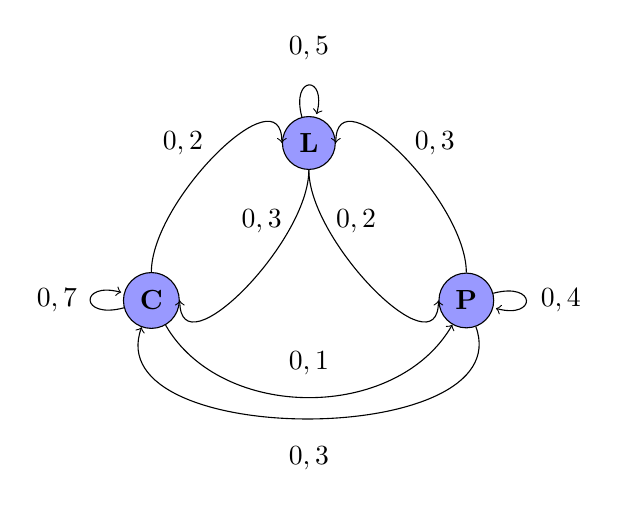
\begin{tikzpicture}
		\node[draw,circle,fill=blue!40!white](L) at (0,2) {\textbf{L}};
		\node[draw,circle,fill=blue!40!white](C) at (-2,0) {\textbf{C}};
		\node[draw,circle,fill=blue!40!white](P) at (2,0) {\textbf{P}};
		\node[draw=none] at (-3.2,0) {$0,7$};
		\node[draw=none] at (-1.6,2) {$0,2$};
		\node[draw=none] at (0,-0.8) {$0,1$};
		\node[draw=none] at (3.2,0) {$0,4$};
		\node[draw=none] at (1.6,2) {$0,3$};
		\node[draw=none] at (0,-2) {$0,3$};
		\node[draw=none] at (0,3.2) {$0,5$};
		\node[draw=none] at (-0.6,1) {$0,3$};
		\node[draw=none] at (0.6,1) {$0,2$};
		\draw[->] (L.south) to [out=-90,in=-90] (P.west);
		\draw[->] (L.south) to [out=-90,in=-90] (C.east);
		\draw[->] (C) to [out=90,in=90] (L.west);
		\draw[->] (C) to [out=-60,in=-120] (P);
		\draw[->] (P) to [out=-70,in=-110] (C);
		\draw[->] (P) to [out=90,in=90] (L.east);
		\draw[->] (L) edge [loop above] ();
		\draw[->] (C) edge [loop left] ();
		\draw[->] (P) edge [loop right] ();
	\end{tikzpicture}
\end{document}
